\documentclass[Chap2main.tex]{subfiles}

% Load any packages needed for this document

\begin{document}
\subsection{Bland-Altman plots}

In light of shortcomings associated with scatterplots,
\citet*{BA83} recommend a further analysis of the data. Firstly
case-wise differences of measurements of two methods $d_{i} =
y_{1i}-y_{2i} \mbox{ for }i=1,2,\dots,n$ on the same subject
should be calculated, and then the average of those measurements
($a_{i} = (y_{1i} + y_{2i})/2 \mbox{ for }i=1,2,\dots, n$).

\citet{BA83} proposes a scatterplot of the case-wise averages and differences of two methods of measurement. This scatterplot has since become widely known as the Bland-Altman plot. \citet*{BA83} express the
motivation for this plot thusly:
\begin{quote}
	``From this type of plot it is much easier to assess the magnitude
	of disagreement (both error and bias), spot outliers, and see
	whether there is any trend, for example an increase in (difference) for high values. This way of plotting the data is a very powerful way of displaying the results of a method comparison study."
\end{quote}

The case wise-averages capture several aspects of the data, such as expressing the range over which the values were taken, and assessing whether the assumptions of constant variance holds.
Case-wise averages also allow the case-wise differences to be presented on a two-dimensional plot, with better data visualization qualities than a one dimensional plot. \citet{BA86}
cautions that it would be the difference against either measurement value instead of their average, as the difference relates to both value. This methodology has proved very popular, and the Bland-Altman plots is widely regarded as powerful graphical methodology for making a visual assessment of the data.

The magnitude of the inter-method bias between the two methods is simply the average of the differences $\bar{d}$. This inter-method bias is represented with a line on the Bland-Altman plot. As the objective of the Bland-Altman plot is to advise on the agreement of two methods, it is the case-wise differences that are also particularly relevant. The variances around this bias is estimated by the standard deviation of these differences $S_{d}$.

\subsection{Bland-Altman plots for the Grubbs data}

In the case of the Grubbs data the inter-method bias is $-0.61$ metres per second, and is indicated by the dashed line on Figure 1.2. By inspection of the plot, it is also possible to compare the precision of each method. Noticeably the differences tend to increase as the averages increase.


The Bland-Altman plot for comparing the `Fotobalk' and `Counter'
methods, which shall henceforth be referred to as the `F vs C'
comparison,  is depicted in Figure 1.2, using data from Table 1.3.
The presence and magnitude of the inter-method bias is indicated
by the dashed line.
\newpage

%Later it will be shown that case-wise differences are the sole
%component of the next part of the methodology, the limits of
%agreement.


\begin{table}[h!]
	\renewcommand\arraystretch{0.7}%
	\begin{center}
		\begin{tabular}{|c||c|c||c|c|}
			\hline
			Round & Fotobalk  & Counter  & Differences  & Averages  \\
			&  [F] & [C] & [F-C] &  [(F+C)/2] \\
			\hline
			1 & 793.8 & 794.6 & -0.8 & 794.2 \\
			2 & 793.1 & 793.9 & -0.8 & 793.5 \\
			3 & 792.4 & 793.2 & -0.8 & 792.8 \\
			4 & 794.0 & 794.0 & 0.0 & 794.0 \\
			5 & 791.4 & 792.2 & -0.8 & 791.8 \\
			6 & 792.4 & 793.1 & -0.7 & 792.8 \\
			7 & 791.7 & 792.4 & -0.7 & 792.0 \\
			8 & 792.3 & 792.8 & -0.5 & 792.5 \\
			9 & 789.6 & 790.2 & -0.6 & 789.9 \\
			10 & 794.4 & 795.0 & -0.6 & 794.7 \\
			11 & 790.9 & 791.6 & -0.7 & 791.2 \\
			12 & 793.5 & 793.8 & -0.3 & 793.6 \\
			\hline
		\end{tabular}
		\caption{Fotobalk and Counter methods: differences and averages.}
	\end{center}
\end{table}

\begin{table}[h!]
	\renewcommand\arraystretch{0.7}%
	\begin{center}
		\begin{tabular}{|c||c|c||c|c|}
			\hline
			Round & Fotobalk  & Terma  & Differences  & Averages  \\
			&  [F] & [T] & [F-T] &  [(F+T)/2] \\
			\hline
			1 & 793.8 & 793.2 & 0.6 & 793.5 \\
			2 & 793.1 & 793.3 & -0.2 & 793.2 \\
			3 & 792.4 & 792.6 & -0.2 & 792.5 \\
			4 & 794.0 & 793.8 & 0.2 & 793.9 \\
			5 & 791.4 & 791.6 & -0.2 & 791.5 \\
			6 & 792.4& 791.6 & 0.8 & 792.0 \\
			7 & 791.7 & 791.6 & 0.1 & 791.6 \\
			8 & 792.3 & 792.4 & -0.1 & 792.3 \\
			9 & 789.6 & 788.5 & 1.1 & 789.0 \\
			10 & 794.4 & 794.7 & -0.3 & 794.5 \\
			11 & 790.9 & 791.3 & -0.4 & 791.1 \\
			12 & 793.5 & 793.5 & 0.0 & 793.5 \\
			
			\hline
		\end{tabular}
		\caption{Fotobalk and Terma methods: differences and averages.}
	\end{center}
\end{table}

\newpage

\begin{figure}[h!]
	\begin{center}
		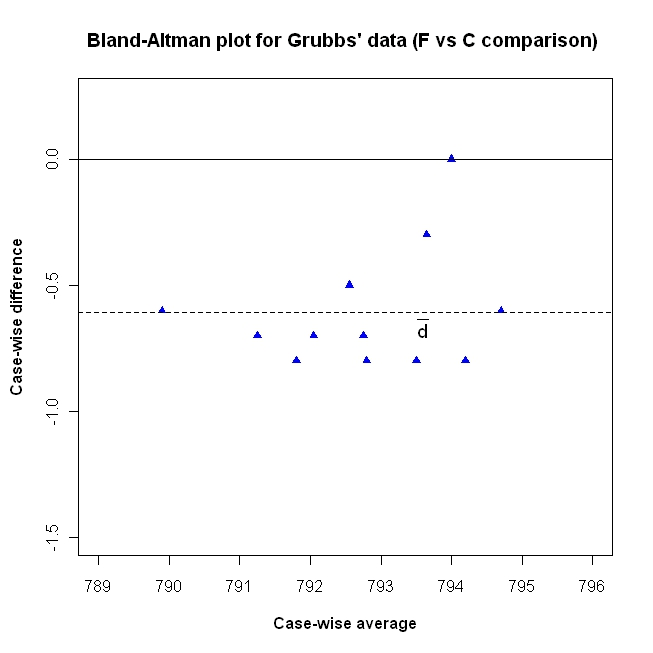
\includegraphics[width=120mm]{GrubbsBAplot-noLOA.jpeg}
		\caption{Bland-Altman plot For Fotobalk and Counter methods.}\label{GrubbsBA-noLOA}
	\end{center}
\end{figure}



In Figure 1.3 Bland-Altman plots for the `F vs C' and `F vs T'
comparisons are shown, where `F vs T' refers to the comparison of
the `Fotobalk' and `Terma' methods. Usage of the Bland-Altman plot
can be demonstrate in the contrast between these comparisons. By inspection, there exists a larger inter-method bias in the `F vs C' comparison than in the `F vs T' comparison. Conversely there
appears to be less precision in `F vs T' comparison, as indicated
by the greater dispersion of covariates.

\begin{figure}[h!]
	\begin{center}
		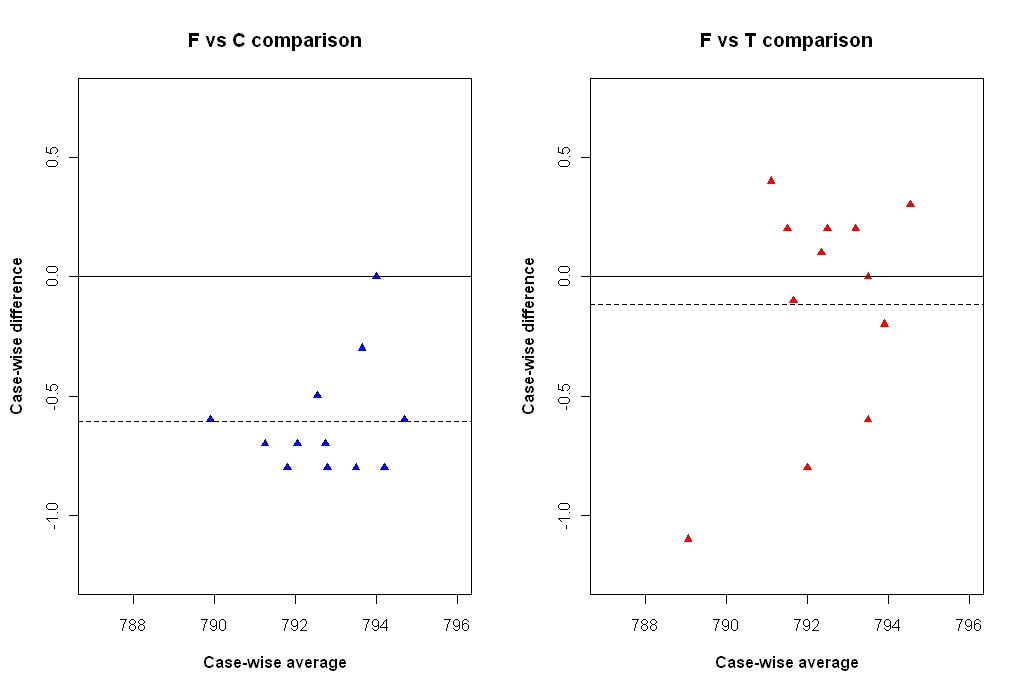
\includegraphics[height=90mm]{GrubbsDataTwoBAplots.jpeg}
		\caption{Bland-Altman plots for Grubbs' F vs C and F vs T comparisons.}\label{GrubbsDataTwoBAplots}
	\end{center}
\end{figure}

\newpage

\subsection{Prevalence of the Bland-Altman plot}
\citet*{BA86}, which further develops the Bland-Altman methodology,
was found to be the sixth most cited paper of all time by the
\citet{BAcite}. \cite{Dewitte} describes the rate at which
prevalence of the Bland-Altman plot has developed in scientific
literature. \citet{Dewitte} reviewed the use of Bland-Altman plots
by examining all articles in the journal `Clinical Chemistry'
between 1995 and 2001. This study concluded that use of the
Bland–Altman plot increased over the years, from 8\% in 1995 to
14\% in 1996, and 31–36\% in 2002.

The Bland-Altman Plot has since become expected, and
often obligatory, approach for presenting method comparison
studies in many scientific journals \citep{hollis}. Furthermore
\citet{BritHypSoc} recommend its use in papers pertaining to
method comparison studies for the journal of the British
Hypertension Society.

\subsection{Adverse features}

Estimates for inter-method bias and variance of differences are only meaningful if there is uniform inter-bias and variability throughout the range of measurements. Fulfilment of these assumptions can be checked by visual inspection of the plot.The prototype Bland-Altman plots depicted in Figures 1.4, 1.5 and 1.6 are derived from simulated data, for the purpose of demonstrating how the plot would inform an analyst of features that would adversely affect use of the recommended methodology.

Figure 1.4 demonstrates how the Bland-Altman plot would indicate
increasing variance of differences over the measurement range.
Fitted regression lines, for both the upper and lower half of the
plot, has been added to indicate the trend. Figure 1.5 is an
example of cases where the inter-method bias changes over the
measurement range. This is known as proportional bias, and is
defined by \citet{ludbrook97} as meaning that `one method gives
values that are higher (or lower) than those from the other by an
amount that is proportional to the level of the measured
variable'. In both Figures 1.4 and 1.5, the assumptions necessary
for further analysis using the limits of agreement are violated.

Application of regression techniques to the Bland-Altman plot, and
subsequent formal testing for the constant variability of
differences is informative. The data set may be divided into two
subsets, containing the observations wherein the difference values
are less than and greater than the inter-method bias respectively.
For both of these fits, hypothesis tests for the respective slopes
can be performed. While both tests can be considered separately,
multiple comparison procedures, such as the Benjamini-Hochberg
\citep{BH} test, should be also be used.

\begin{figure}[h!]
	\begin{center}
		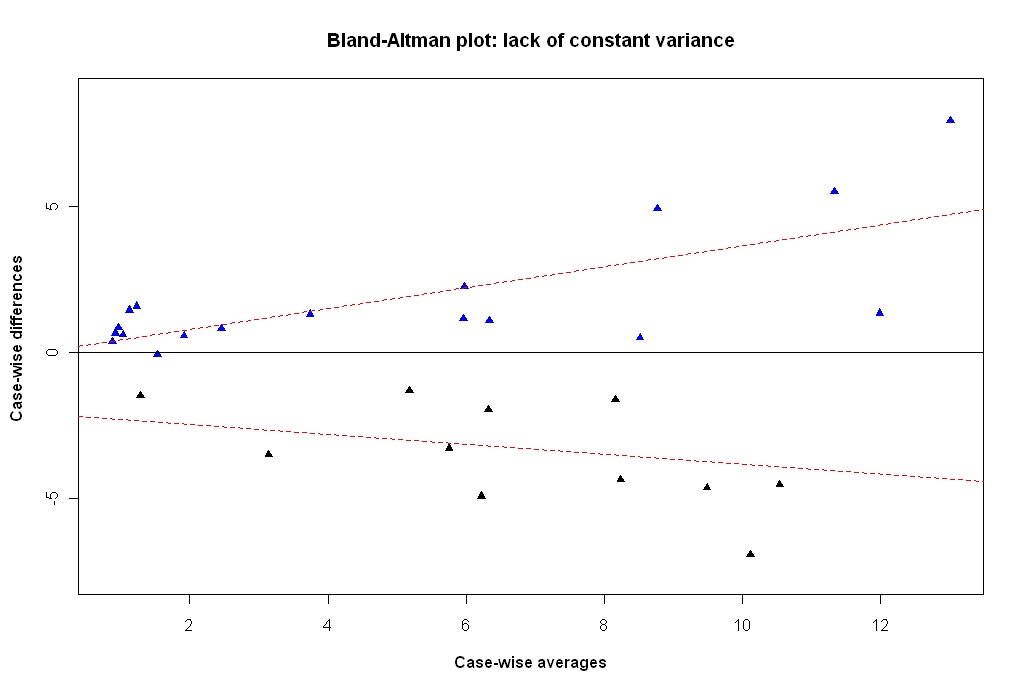
\includegraphics[height=90mm]{BAFanEffect.jpeg}
		\caption{Bland-Altman plot demonstrating the increase of variance over the range.}\label{BAFanEffect}
	\end{center}
\end{figure}

\begin{figure}[h!]
	\begin{center}
		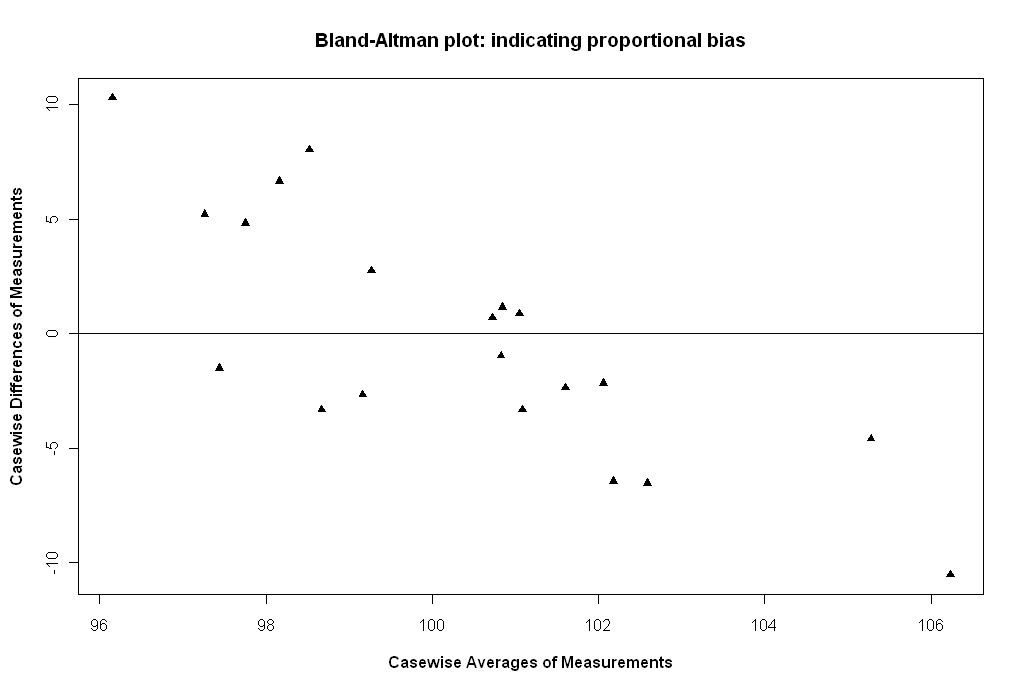
\includegraphics[height=90mm]{PropBias.jpeg}
		\caption{Bland-Altman plot indicating the presence of proportional bias.}\label{PropBias}
	\end{center}
\end{figure}

\begin{figure}[h!]
	\begin{center}
		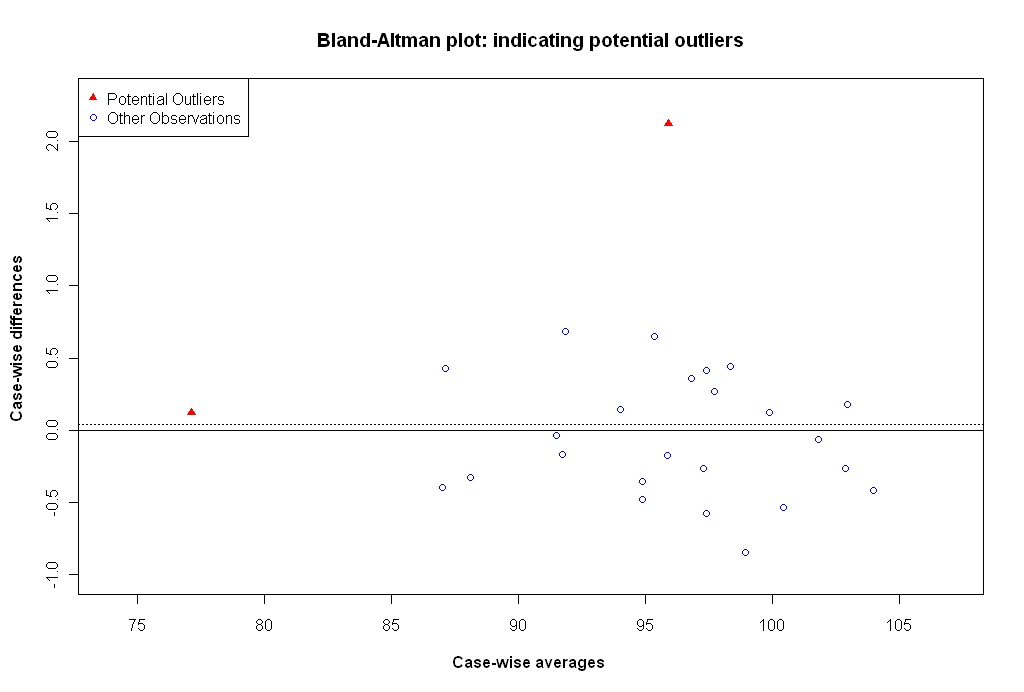
\includegraphics[width=125mm]{BAOutliers.jpeg}
		\caption{Bland-Altman plot indicating the presence of potential outliers.}\label{Outliers}
	\end{center}
\end{figure}

\newpage


The Bland-Altman plot also can be used to identify outliers. An
outlier is an observation that is conspicuously different from the
rest of the data that it arouses suspicion that it occurs due to a
mechanism, or conditions, different to that of the rest of the
observations. \citet*{BA99} do not recommend excluding outliers from analyzes,
but remark that recalculation of the inter-method bias estimate,
and further calculations based upon that estimate, are useful for
assessing the influence of outliers. The authors remark that `we
usually find that this method of analysis is not too sensitive to
one or two large outlying differences'. Figure 1.6 demonstrates how the Bland-Altman
plot can be used to visually inspect the presence of potential
outliers.

As a complement to the Bland-Altman plot, \citet{Bartko} proposes
the use of a bivariate confidence ellipse, constructed for a
predetermined level. \citet{AltmanEllipse} provides the relevant calculations for the
ellipse. This ellipse is intended as a visual
guidelines for the scatter plot, for detecting outliers and to
assess the within- and between-subject variances.

The minor axis relates to the between subject variability, whereas
the major axis relates to the error mean square, with the ellipse
depicting the size of both relative to each other.
Consequently Bartko's ellipse provides a visual aid to determining the
relationship between variances. If $\mbox{var}(a)$ is greater than $\mbox{var}(d)$, the orientation of the ellipse is horizontal. Conversely if $\mbox{var}(a)$ is less than $\mbox{var}(d)$, the orientation of the ellipse is vertical.


%(Furthermore \citet{Bartko}
%proposes formal testing procedures, that shall be discussed in due
%course.)

The Bland-Altman plot for the Grubbs data, complemented by Bartko's ellipse, is depicted in Figure 1.7.
The fourth observation is shown to be outside the bounds of the ellipse, indicating that it is a potential outlier.


\begin{figure}[h!]
	% Requires \usepackage{graphicx}
	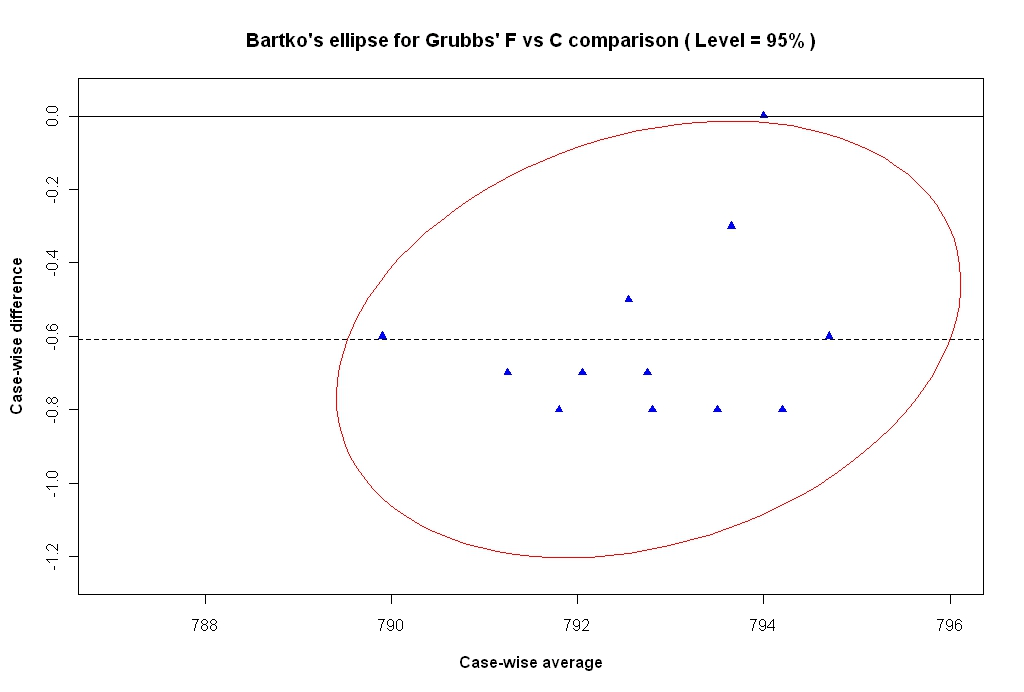
\includegraphics[width=130mm]{GrubbsBartko.jpeg}
	\caption{Bartko's Ellipse For Grubbs' Data.}\label{GrubbsBartko}
\end{figure}

The limitations of using bivariate approaches to outlier detection
in the Bland-Altman plot can demonstrated using Bartko's ellipse.
A covariate is added to the `F vs C' comparison that has a
difference value equal to the inter-method bias, and an average
value that markedly deviates from the rest of the average values
in the comparison, i.e. 786. Table 1.8 depicts a $95\%$ confidence
ellipse for this manipulated data set. By inspection of the
confidence interval, a conclusion would be reached that this extra
covariate is an outlier, in spite of the fact that this
observation is wholly consistent with the conclusion of the
Bland-Altman plot.

\begin{figure}[h!]
	% Requires \usepackage{graphicx}
	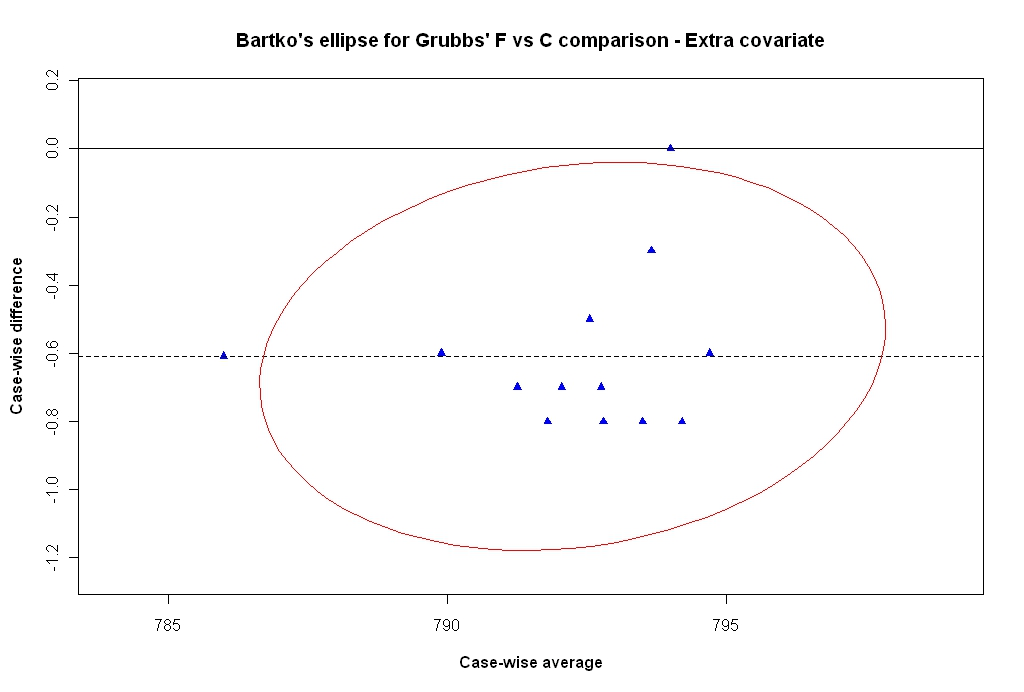
\includegraphics[width=130mm]{GrubbsBartko2.jpeg}
	\caption{Bartko's Ellipse For Grubbs' Data, with an extra covariate.}\label{GrubbsBartko2}
\end{figure}


Importantly, outlier classification must be informed by the logic of the
data's formulation. In the Bland-Altman plot, the horizontal displacement of any
observation is supported by two independent measurements. Any
observation should not be considered an outlier on the basis of a
noticeable horizontal displacement from the main cluster, as in
the case with the extra covariate. Conversely, the fourth
observation, from the original data set, should be considered an
outlier, as it has a noticeable vertical displacement from the
rest of the observations.

%Grubbs' test is a statistical test used for detecting outliers in a
%univariate data set that is assumed to be normally distributed.

%\citet{Grubbs} defined an outlier as a co-variate that appears to
%deviate markedly from other members of the sample in which it
%occurs.

In classifying whether a observation from a univariate data set is
an outlier, many formal tests are available, such as the Grubbs test for outliers. In assessing
whether a covariate in a Bland-Altman plot is an outlier, this
test is useful when applied to the case-wise difference values treated as a
univariate data set. The null hypothesis of the Grubbs test procedure is the absence
of any outliers in the data set. Conversely, the alternative hypotheses is that there is at least one outlier
present.

The test statistic for the Grubbs test ($G$) is the largest
absolute deviation from the sample mean divided by the standard
deviation of the differences,
\[
G =  \displaystyle\max_{i=1,\ldots, n}\frac{\left \vert d_i -
	\bar{d}\right\vert}{S_{d}}.
\]

For the `F vs C' comparison it is the fourth observation gives
rise to the test statistic, $G = 3.64$. The critical value is
calculated using Student's $t$ distribution and the sample size,
\[
U = \frac{n-1}{\sqrt{n}} \sqrt{\frac{t_{\alpha/(2n),n-2}^2}{n - 2
		+ t_{\alpha/(2n),n-2}^2}}.
\]
For this test $U = 0.75$. The conclusion of this test is that the fourth observation in the `F vs C' comparison is an outlier, with $p-$value = 0.003, according with the previous result using Bartko's ellipse.

\newpage



\subsection{Inferences on Bland-Altman estimates}
\citet*{BA99}advises on how to calculate confidence intervals for the inter-method bias and limits of agreement.
For the inter-method bias, the confidence interval is a simply that of a mean: $\bar{d} \pm t_{(0.5\alpha,n-1)} S_{d}/\sqrt{n}$.
The confidence
intervals and standard error for the limits of agreement follow from the variance of the limits of agreement, which is shown to be

\[
\mbox{Var}(LoA) = (\frac{1}{n}+\frac{1.96^{2}}{2(n-1)})s_{d}^{2}.
\]

If $n$ is sufficiently large this can be following approximation
can be used
\[
\mbox{Var}(LoA) \approx 1.71^{2}\frac{s_{d}^{2}}{n}.
\]
Consequently the standard errors of both limits can be
approximated as $1.71$ times the standard error of the
differences.

A $95\%$ confidence interval can be determined, by means of the
\emph{t} distribution with $n-1$ degrees of freedom. However \citet*{BA99} comment that such calculations  may be `somewhat optimistic' on account of the associated assumptions not being realized.

%\subsubsection{Small Sample Sizes} The limits of agreement are
%estimates derived from the sample studied, and will differ from
%values relevant to the whole population, hence the importance of a
%suitably large sample size. A different sample would give
%different limits of agreement. Student's t-distribution is a well
%known probability distribution used in statistical inference for
%normally distributed populations when the sample size is small
%\citep{student,Fisher3}. Consequently, using 't' quantiles , as
%opposed to standard normal quantiles, may give a more appropriate
%calculation for limits of agreement when the sample size is small.
%For sample size $n=12$ the `t' quantile is 2.2 and the limits of
%agreement are (-0.074,-1.143).


\subsection{Formal definition of limits of agreement}
\citet{BA99} note the similarity of limits of agreement to
confidence intervals, but are clear that they are not the same
thing. Interestingly, they describe the limits as `being like a
reference interval'.

Limits of agreement have very similar construction to Shewhart
control limits. The Shewhart chart is a well known graphical
methodology used in statistical process control. Consequently
there is potential for misinterpreting the limits of agreement as
if equivalent to Shewhart control limits. Importantly the
parameters used to determine the Shewhart limits are not based on any sample used for an analysis, but
on the process's historical values, a key difference with
Bland-Altman limits of agreement.

\citet{BXC2008} regards the limits of agreement as a prediction
interval for the difference between future measurements with the
two methods on a new individual, but states that it does not fit
the formal definition of a prediction interval, since the
definition does not consider the errors in estimation of the
parameters. Prediction intervals, which are often used in
regression analysis, are estimates of an interval in which future
observations will fall, with a certain probability, given what has
already been observed. \citet{BXC2008} offers an alternative
formulation, a $95\%$ prediction interval for the difference
\[
\bar{d} \pm t_{(0.975, n-1)}s_{d} \sqrt{1+\frac{1}{n}}
\]

\noindent where $n$ is the number of subjects. Carstensen is
careful to consider the effect of the sample size on the interval
width, adding that only for 61 or more subjects is there a
quantile less than 2.

\citet{luiz} offers an alternative description of limits of
agreement, this time as tolerance limits. A tolerance interval for
a measured quantity is the interval in which a specified fraction
of the population's values lie, with a specified level of
confidence. \citet{Barnhart} describes them as a probability
interval, and offers a clear description of how they should be
used;`if the absolute limit is less than an acceptable difference
$d_{0}$, then the agreement between the two methods is deemed
satisfactory'.

The prevalence of contradictory definitions of what limits of agreement strictly are will inevitably attenuate the poor standard of reporting using limits of agreement, as mentioned by \citet{mantha}.

%At least 100 historical
%values must be used to determine the acceptable value (i.e the
%process mean) and the process standard deviation. The principle
%that the mean and variance of a large sample of a homogeneous
%population is a close approximation of the population's mean and
%variance justifies this.

%\begin{figure}[h!]
%\begin{center}
%  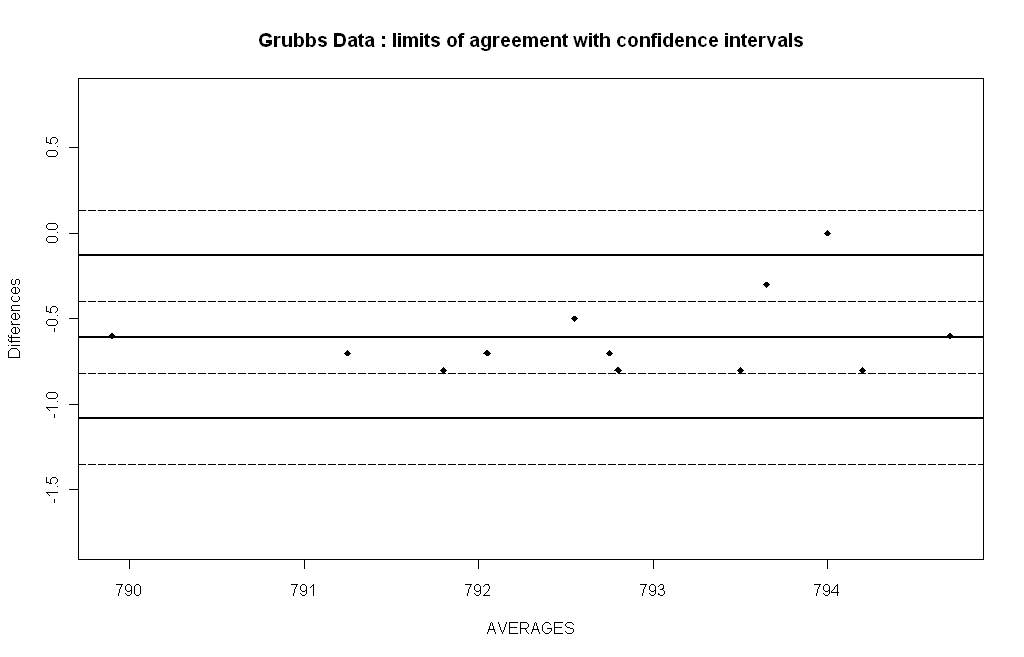
\includegraphics[width=125mm]{GrubbsLOAwCIs.jpeg}
%  \caption{Limits of agreement with confidence intervals}\label{LOAwCIs}
%\end{center}
%\end{figure}

%\newpage
%\section{Agreement Indices}
%\citet{Barnhart} provided an overview of several agreement
%indices, including the limits of agreement. Other approaches, such
%as mean squared deviation, the tolerance deviation index and
%coverage probability are also discussed.




\subsection{Replicate Measurements}

Thus far, the formulation for comparison of two measurement
methods is one where one measurement by each method is taken on
each subject. Should there be two or more measurements by each
methods, these measurement are known as `replicate measurements'.
\citet{BXC2008} recommends the use of replicate measurements, but
acknowledges the additional computational complexity.

\citet*{BA86} address this problem by offering two different
approaches. The premise of the first approach is that replicate
measurements can be treated as independent measurements. The
second approach is based upon using the mean of the each group of
replicates as a representative value of that group. Using either
of these approaches will allow an analyst to estimate the inter
method bias.

%\subsubsection{Mean of Replicates Limits of Agreement}

However, because of the removal of the effects of the replicate
measurements error, this would cause the estimation of the
standard deviation of the differences to be unduly small.
\citet*{BA86} propose a correction for this.

\citet{BXC2008} takes issue with the limits of agreement based on
mean values of replicate measurements, in that they can only be interpreted as prediction
limits for difference between means of repeated measurements by
both methods, as opposed to the difference of all measurements.
Incorrect conclusions would be caused by such a misinterpretation.
\citet{BXC2008} demonstrates how the limits of agreement
calculated using the mean of replicates are `much too narrow as
prediction limits for differences between future single
measurements'. This paper also comments that, while treating the
replicate measurements as independent will cause a downward bias
on the limits of agreement calculation, this method is preferable
to the `mean of replicates' approach.


\subsection{Bland-Altman correlation test}

The approach proposed by \citet{BA83} is a formal test on the
Pearson correlation coefficient of case-wise differences and means
($\rho_{AD}$). According to the authors, this test is equivalent
to the `Pitman Morgan Test'. For the Grubbs data, the correlation
coefficient estimate ($r_{AD}$) is 0.2625, with a 95\% confidence
interval of (-0.366, 0.726) estimated by Fishers `$r$ to $z$'
transformation \citep*{Cohen}. The null hypothesis ($\rho_{AD}$ =0)
fail to be rejected. Consequently the null hypothesis of equal
variances of each method would also fail to be rejected. There has
no been no further mention of this particular test in
\citet{BA86}, although \citet{BA99} refers to Spearman's rank
correlation coefficient. \citet{BA99} comments `we do not see a
place for methods of analysis based on hypothesis testing'.
\citet{BA99} also states that consider structural equation models
to be inappropriate.

\subsection{Identifiability}
\citet{DunnSEME} highlights an important issue regarding using
models such as these, the identifiability problem. This comes as a
result of there being too many parameters to be estimated.
Therefore assumptions about some parameters, or estimators used,
must be made so that others can be estimated. For example in literature the variance
ratio $\lambda=\frac{\sigma^{2}_{1}}{\sigma^{2}_{2}}$
must often be assumed to be equal to $1$ \citep{linnet98}.\citet{DunnSEME} considers methodologies based on two methods with single measurements on each subject as inadequate for a serious
study on the measurement characteristics of the methods. This is
because there would not be enough data to allow for a meaningful
analysis. There is, however, a contrary argument that in many
practical settings it is very difficult to get replicate
observations when the measurement method requires invasive medical
procedure.

%%%%%%%%%%%%%%%%%%%%%%%%%%%%%%%%%%%%%%%%%%%%%%%%%%%%%%%%%%%%%%%%%%%%%%%%%%%%%%%Bartko's BB
\citet{BB89} offers a formal simultaneous hypothesis test for the
mean and variance of two paired data sets. Using simple linear
regression of the differences of each pair against the sums, a
line is fitted to the model, with estimates for intercept and
slope ($\hat{\beta}_{0}$ and $\hat{\beta}_{1}$). The null
hypothesis of this test is that the mean ($\mu$) and variance
($\sigma^{2}$) of both data sets are equal if the slope and
intercept estimates are equal to zero(i.e $\sigma^{2}_{1} =
\sigma^{2}_{2}$ and $\mu_{1}=\mu_{2}$ if and only if $\beta_{0}=
\beta_{1}=0$ )

A test statistic is then calculated from the regression analysis
of variance values \citep{BB89} and is distributed as `$F$' random
variable. The degrees of freedom are $\nu_{1}=2$ and $\nu_{1}=n-2$
(where $n$ is the number of pairs). The critical value is chosen
for $\alpha\%$ significance with those same degrees of freedom.
\citet{Bartko} amends this methodology for use in method
comparison studies, using the averages of the pairs, as opposed to
the sums, and their differences. This approach can facilitate
simultaneous usage of test with the Bland-Altman methodology.
Bartko's test statistic take the form:
\[ F.test = \frac{(\Sigma d^{2})-SSReg}{2MSReg}
\]
% latex table generated in R 2.6.0 by xtable 1.5-5 package
% Mon Aug 31 15:53:51 2009
\begin{table}[ht]
	\begin{center}
		\begin{tabular}{lrrrrr}
			\hline
			& Df & Sum Sq & Mean Sq & F value & Pr($>$F) \\
			\hline
			Averages & 1 & 0.04 & 0.04 & 0.74 & 0.4097 \\
			Residuals & 10 & 0.60 & 0.06 &  &  \\
			\hline
		\end{tabular}
		\caption{Regression ANOVA of case-wise differences and averages
			for Grubbs Data}
	\end{center}
\end{table}
%(calculate using R code $qf(0.95,2,10)$).

For the Grubbs data, $\Sigma d^{2}=5.09 $, $SSReg = 0.60$ and
$MSreg=0.06$ Therefore the test statistic is $37.42$, with a
critical value of $4.10$. Hence the means and variance of the
Fotobalk and Counter chronometers are assumed to be simultaneously
equal.

Importantly, this methodology determines whether there is both
inter-method bias and precision present, or alternatively if there
is neither present. It has previously been demonstrated that there
is a inter-method bias present, but as this procedure does not
allow for separate testing, no conclusion can be drawn on the
comparative precision of both methods.



%This application of the
%Grubbs method presumes the existence of this condition, and necessitates
%replication of observations by means external to and independent of the first
%means. The Grubbs estimators method is based on the laws of propagation of
%error. By making three independent simultaneous measurements on the same
%physical material, it is possible by appropriate mathematical manipulation of
%the sums and differences of the associated variances to obtain a valid
%estimate of the precision of the primary means. Application of the Grubbs
%estimators procedure to estimation of the precision of an apparatus uses
%the results of a physical test conducted in such a way as to obtain a series
%of sets of three independent observations.


\section{Regression Methods}
Conventional regression models are estimated using the ordinary
least squares (OLS) technique, and are referred to as `Model I
regression' \citep{CornCoch,ludbrook97}. A key feature of Model I
models is that the independent variable is assumed to be measured
without error. As often pointed out in several papers
\citep{BA83,ludbrook97}, this assumption invalidates simple linear
regression for use in method comparison studies, as both methods
must be assumed to be measured with error.

The use of regression models that assumes the presence of error in
both variables $X$ and $Y$ have been proposed for use instead
\citep{CornCoch,ludbrook97}. These methodologies are collectively
known as `Model II regression'. They differ in the method used to
estimate the parameters of the regression.

Regression estimates depend on formulation of the model. A
formulation with one method considered as the $X$ variable will
yield different estimates for a formulation where it is the $Y$
variable. With Model I regression, the models fitted in both cases
will entirely different and inconsistent. However with Model II
regression, they will be consistent and complementary.

Regression approaches are useful for a making a detailed examination of the biases across the range of measurements, allowing bias to be decomposed into fixed bias and proportional bias.
Fixed bias describes the case where one method gives values that are consistently different
to the other across the whole range. Proportional
bias describes the difference in measurements getting progressively greater, or smaller, across the range of measurements. A measurement method may have either an attendant fixed bias or proportional bias, or both. \citep{ludbrook}. Determination of these biases shall be discussed in due course.

\section{Limits of Agreement}

Computing limits of agreement features prominently in many method comparison studies, further to \citet{BA86,BA99}.
\citet{BA99} addresses the issue of computing LoAs in the presence of replicate measurements, suggesting several computationally simple approaches. When repeated measures data are available, it is desirable to use
all the data to compare the two methods. However, the original Bland-Altman method was developed for two sets of measurements done on one occasion (i.e. independent data), and so this approach is not suitable for replicate measures data. However, as a naive analysis, it may be used to explore the data because of the simplicity of the method.
\citet{bxc2008}  computes the limits of agreement to the case with replicate measurements by using LME models.

\section{Outline of Thesis}
Thus the study of method comparison is introduced. The intention of this thesis is to progress the
study of method comparison studies, using a statistical method known as Linear mixed effects models.
Chapter two shall describe linear mixed effects models, and how the use of the linear mixed
effects models have so far extended to method comparison studies. Implementations of important existing work shall be presented, using the \texttt{R} programming language.

Model diagnostics are an integral component of a complete statistical analysis.
In chapter three model diagnostics shall be described in depth, with particular
emphasis on linear mixed effects models, further to chapter two.

For the fourth chapter, important linear mixed effects model diagnostic methods shall be extended to method comparison studies, and proposed methods shall be demonstrated on data sets that have become well known in literature on method comparison. The purpose is to both calibrate these methods and to demonstrate applications for them.
The last chapter shall focus on robust measures of important parameters such as agreement.

\bibliography{DB-txfrbib}
\end{document}
